\documentclass{article}
\usepackage[utf8]{inputenc}
\usepackage[margin=0.8in]{geometry}
\usepackage{graphicx}
\usepackage{wrapfig}

\usepackage{natbib}
\usepackage{graphicx}
% Para los codigos
\usepackage{listings}
\usepackage[spanish]{babel}
\usepackage[hidelinks]{hyperref}
\usepackage{lscape}

\lstset{
basicstyle=\ttfamily,
frame=single,
language=SQL,
tabsize=2,
literate=%
    {á}{{\'a}}1
    {é}{{\'e}}1
    {è}{{\`e}}1
    {í}{{\'i}}1
    {ó}{{\'o}}1
    {ú}{{\'u}}1
}
\begin{document}

\begin{titlepage}
	\title{
		\begin{Huge}
			Practica 3 - BASES DE DATOS 2
		\end{Huge}
	}
	\author{
	  Hayk Kocharyan\\
	  757715@unizar.es
	  \and
	  Juan José Tambo Tambo\\
	  755742@unizar.es
	  \and
	  Pedro Tamargo Allué\\
	  758267@unizar.es
	  \and
	  Jesús Villacampa Sagaste\\
	  755739@unizar.es
	}
	\date{\today}
	
	\clearpage\maketitle
	\thispagestyle{empty}
	\tableofcontents

\end{titlepage}

\newpage 

\section{Esfuerzos invertidos}
Los esfuerzos invertidos por cada integrante del equipo son:
\begin{itemize}
\item Hayk:

\item Juanjo:	

\item Jesús:

\item Pedro: 

\end{itemize}

\section{Parte 1 - Esquema conceptual y lógico de la base de datos relacional diseñada en la práctica anterior}

\textbf{Mostrar aqui el ER de la práctica anterior y contar su traducción a SQL diciendo las decisiones de diseño de forma DETALLADA.}

Durante el desarrollo de la práctica 1 se diseñó una base de datos para un banco que quería gestionar cuentas con múltiples propietarios, diferentes tipos de cuentas (cuentas ahorro y cuentas corrientes), operaciones (transacciones entre cuentas, o movimientos de dinero en efectivo) y las sucursales de la entidad.\\
En la Figura \ref{fig:er1} se puede observar el esquema entidad relación sobre el problema planteado. Se ha planteado las relaciones entre los distintos tipos de cuentas como una generalización, ya que todas comparten ciertos atributos como el número de cuenta, el \emph{IBAN}, la fecha de apertura y el saldo restante. Esta generalización es exclusiva ya que no se considera posible la capacidad de que una cuenta pertenezca a los dos tipos de entidades al mismo tiempo. También, se trata de una generalización total ya que no se considera el caso de que una cuenta no pertenezca a algunos de las entidades derivadas de \emph{Cuenta}.\\
Con transacción ocurre lo mismo, una transferencia entre cuentas y las operaciones de retirada o ingreso de efectivo se pueden generalizar en una nueva entidad \emph{Transacción} con los atributos comunes a ambas entidades, tales como: el número de la transacción, la fecha y hora de la misma, su importe y una descripción a modo de concepto. Se trata de una generalización exclusiva ya que una transferencia no puede pertenecer a los dos subtipos a la vez. También, se trata de una generalización total ya que en el contexto del problema no tiene sentido que exista una transferencia que no pertenezca a \emph{Operación (operaciones en efectivo)} o a \emph{Transferencia (transferencia de saldo entre cuentas)}.\\
Se ha decidido que \emph{Transacción} debía ser débil respecto a \emph{cuenta} ya que depende en existencia e identificación de \emph{cuenta}, por lo tanto la relación \emph{Realizar} es una relación \emph{1:N} entre \emph{Cuenta} y \emph{Transacción}. No obstante, existe una transacción que no indica la debilidad de la entidad \emph{Transacción} respecto a \emph{Cuenta}, la relación \emph{Recibir}, una relación \emph{1:N} que relaciona las entidades \emph{Cuenta} y \emph{Transferencia} , y cuyo significado es relacionar una transferencia con la cuenta beneficiaria.\\
Los clientes titulares de una cuenta se reflejan en la entidad \emph{Cliente}, que almacena el DNI, el nombre, los apellidos la dirección y el email. Se ha decidido que el \emph{DNI} sea la clave primaria ya que es único para los ciudadanos.\\
La relación de \emph{Cliente} con \emph{Cuenta} se encuentra en \emph{Poseer}, una relación \emph{M:N} que posibilita que una cuenta tenga más de un titular.\\
Para el almacenamiento de las sucursales de la entidad bancaria, se ha diseñado una entidad \emph{Sucursal}, que almacena el código de la entidad, su dirección postal y el teléfono de la oficina. Se ha decidido que el código de la sucursal sea la clave primaria que identifique a las sucursales ya que dentro de la misma entidad bancaria no existen dos sucursales con el mismo código.\\
Se ha considerado que las transacciones se tienen que realizar en una sucursal, por lo tanto existe una relación entre \emph{Transacción} y \emph{Sucursal}. También, una cuenta corriente debe ser abierta en una determinada sucursal de la entidad.\\

En la traducción de las generalizaciones del esquema conceptual al esquema lógico (modelo relacional) se han escogido dos estrategias. En la generalización de \emph{Cuenta} se ha mantenido la entidad, y las entidades derivadas de la misma solamente almacenan los atributos necesarios que no pertenecen a \emph{Cuenta}.\\
Por otra parte, en la generalización de \emph{Transacción} se ha optado por eliminar la entidad generalizada, obteniendo así dos entidades independientes y duplicando algunos de sus atributos. \textbf{Leyendo esto me doy cuenta que nos hacía falta un \emph{Trigger}}. En esta misma generalización se ha traducido la relación \emph{1:N} entre \emph{Cuenta} y \emph{Transacción} como un atributo (el número de cuenta) en la tablas derivadas de \emph{Transacción} \textbf{TODO: Esto no se cuanto de bien está redactado}, siendo una referencia a la cuenta que ha realizado la transacción.\\
{\LARGE \textbf{¿CÓMO LES PONEMOS EL ESQUEMA LÓGICO? Un diagrama?}}

\section{Parte 1 - Determinación del esquema lógico y conceptual de la base de datos Oracle a integrar}

\textbf{Esquema ER de la base de datos a integrar y PONER LAS CONSULTAS CON LAS QUE HEMOS SACADO LAS COSAS.}\\
\textbf{Igual estaría bien comentar de donde hemos sacado la información.}

En esta práctica se pide integrar la base de datos de la Práctica 1+2 en otra base de datos ya existente (\emph{Banquete}). Para ello, es preciso conocer la organización de sus tablas y como se relacionan unas con otras, por tanto, el primer paso para conseguir la integración es extraer toda la información posible de la base de datos de \emph{Banquete}.\\
\emph{Banquete} es una base de datos proporcionada por los profesores de la asignatura y se puede acceder a ella a través de las máquinas del laboratorio. Al conectarse a \emph{lab000} y ejecutar el comando \emph{sqlplus2 aNIP@barret.danae04.unizar.es} (siendo NIP el identificador de la universidad de cada miembro) e introduciendo la contraseña proporcionada en el fichero \emph{README-oracle2}, cada componente del grupo tiene acceso a Oracle con la base de datos \emph{Banquete} ya cargada.\\
Una vez conseguido el acceso a \emph{Banquete}, a través de las consultas expuestas a continuación se consigue toda la información sobre tablas, vistas, triggers o constraints necesarios para conocer el funcionamiento al completo de la misma. 

\textbf{TODO Hay que insertar todas consultas que hicimos CREO QUE FALTAN}

\begin{lstlisting}
	-- Obtenemos las tablas
	SELECT table_name FROM user_tables@SCHEMA2BD2;
	-- Describir los atributos de la tabla <nombre_tabla>
	DESC <nombre_tabla>@SCHEMA2BD2;

	-- Para obtener las restricciones (clave primaria, ajena,
	--  restricciones de consistencia) para una tabla <nombre_tabla>
	SELECT UCC.CONSTRAINT_NAME, UCC.COLUMN_NAME, UC.CONSTRAINT_TYPE, 
	 UC.SEARCH_CONDITION, UC2.TABLE_NAME as REFERENCES_TABLE
	FROM USER_CONS_COLUMNS@SCHEMA2BD2 UCC, USER_CONSTRAINTS@SCHEMA2BD2 UC,
	 USER_CONSTRAINTS@SCHEMA2BD2 UC2
	WHERE UCC.CONSTRAINT_NAME = UC.CONSTRAINT_NAME
	AND UC.R_CONSTRAINT_NAME = UC2.CONSTRAINT_NAME(+)
	AND UCC.TABLE_NAME = '<nombre_tabla>'
	ORDER BY UCC.CONSTRAINT_NAME;
	
	-- Para obtener las vistas de la base de datos a integrar
	SELECT UV.VIEW_NAME, UV.TEXT, UTC.COMMENTS
	FROM USER_VIEWS@SCHEMA2BD2 UV, USER_TAB_COMMENTS@SCHEMA2BD2 UTC
	WHERE UV.VIEW_NAME = UTC.TABLE_NAME(+);
	
	-- Para obtener los triggers
	SELECT TRIGGER_NAME, TRIGGER_TYPE, TRIGGERING_EVENT, TABLE_NAME,
	 WHEN_CLAUSE, DESCRIPTION, TRIGGER_BODY
	FROM USER_TRIGGERS@SCHEMA2BD2;
\end{lstlisting}

\textbf{Comprobar si quereis mover este párrafo}\\
Para la extracción de la información con las consultas anteriores se ha utilizado la herramienta \emph{spool} y \emph{DBeaver}. Con estas herramientas se ha extraido la información sobre la estructura de la base de datos de \emph{Banquete} de una forma tabular (en ficheros .csv), facilitando su comprensión, ya que, utilizando la terminal la salida obtenida era difícil de interpretar.\\

Una vez conseguida toda la información, se necesita crear un modelo conceptual canónico de \emph{Banquete} con el fin de poder crear a continuación el esquema global que las dos bases. La transformación de las tablas a un modelo E/R es prácticamente directo gracias a los constraints que proporcionan la información de claves primarias y ajenas de las que se pueden sacar la manera en la que están relacionadas las tablas. Una vez procesada y analizada la información obtenida se obtiene el siguiente esquema E/R \ref{fig:er_banquete}.

\section{Parte 1 - Mejoras sugeridas para la base de datos a integrar}\label{mejoras}

Durante el interrogatorio al catálogo de datos de la base de datos de \emph{Banquete} se han encontrado diversas anomalías y diferencias respecto a nuestra base de datos.\\
En la base de datos a integrar una cuenta solo puede disponer de un titular. Además en \emph{Titular} (se corresponde con \emph{Cliente} de \emph{Banquito}), no dispone de un atributo destinado para la dirección, si no que cuenta con una clave ajena a una entidad \emph{Dirección}, que no está relacionada con su entidad \emph{CodPostal}. Esta entidad \emph{CodPostal} almacena: calle, ciudad y código postal, por lo tanto a partir de una dirección si que se puede obtener su código postal pero al no estar relacionado habría que realizar consultas extras y a la par de que la información se encuentra duplicada en dos tablas de la base de datos (calle y ciudad).\\
La entidad \emph{Sucursal} no dispone de un atributo como clave ajena de \emph{Dirección}, en este caso solamente se dispone de una restricción de consistencia sobre su valor que comprueba que este atributo no sea \emph{NULL}. Esto puede duplicar la información existente en \emph{Dirección} y en este atributo \emph{Dir}.\\
En la entidad \emph{CodEntidades} encontramos el problema de que no está relacionada con ninguna otra. En este caso no duplica información y en ella se encuentran los códigos de las distintas entidades bancarias conocidas por el sistema de cuentas de \emph{Banquete}.\\
La entidad \emph{OpTransferencia} tiene un atributo destinado a albergar el número de cuenta corriente de la cuenta destino, no obstante, al igual que con \emph{Sucursal}, este atributo no es una clave ajena de una \emph{Cuenta}. Esto puede ser debido a que \emph{Banquete} (transferencia entre \emph{Banquete} y \emph{Banco Generosidad}) ofrece la posibilidad de realizar transferencias entre cuentas que no tienen porque pertenecer a su entidad. Este aspecto no se tuvo en cuenta a la hora de diseñar la base de datos de \emph{Banquito}.\\
Un problema similar existe en la entidad \emph{OpEfectivo}, ya que tiene un atributo destinado a identificar la \emph{Sucursal} en la que se ha realizado una operación con dinero en efectivo, pero este campo no se trata de una restricción de integridad referencial (clave ajena) si no que se trata de una restricción de consistencia que se impide que este campo sea \emph{NULL}.\\
Sobre la generalización de \emph{Cuenta} en \emph{CuentaCorriente} y \emph{CuentaAhorro} se ha descubierto que en la base de datos de \emph{Banquete} no se trata de una generalización disjunta si no que existen cuentas que pueden pertenecer a ambos tipos al mismo tiempo.\\


\textbf{Hablar aquí de los problemas que hemos encontrado y lo que supone que esté mal.}

\section{Parte 1 - Definición e implementación del esquema global en Oracle}

\textbf{Se me ocurre que podríamos explicar lo de que no ponemos como una entidad aparte lo de \emph{Dirección} exponiendo que no queríamos ``romper'' el mal trabajo que hicieron con \emph{Sucursal} y que queríamos unificarlo.}
\textbf{Poner aquí el esquema ER y decir las decisiones de diseño (y el por qué).}\\

Para la elaboración del esquema global se ha realizado un meticuloso estudio del diseño de la base de datos de \emph{Banquete}, centrandose principalemente en las entidades que mas difieren de \emph{Banquito} como se ha explicado detalladamente en \hyperref[mejoras]{el apartado anterior }.\\
A partir de estas diferencias obtenidas se ha realizado el siguiente esquma global:\\
\begin{huge}
SI QUEREIS QUITAD LA IMAGEN, PERO IGUAL ES MAS COMODO PARA QUE SE VEA AL EXPLICARLO Y LEERLO\\
\end{huge}
\begin{figure}
\centering
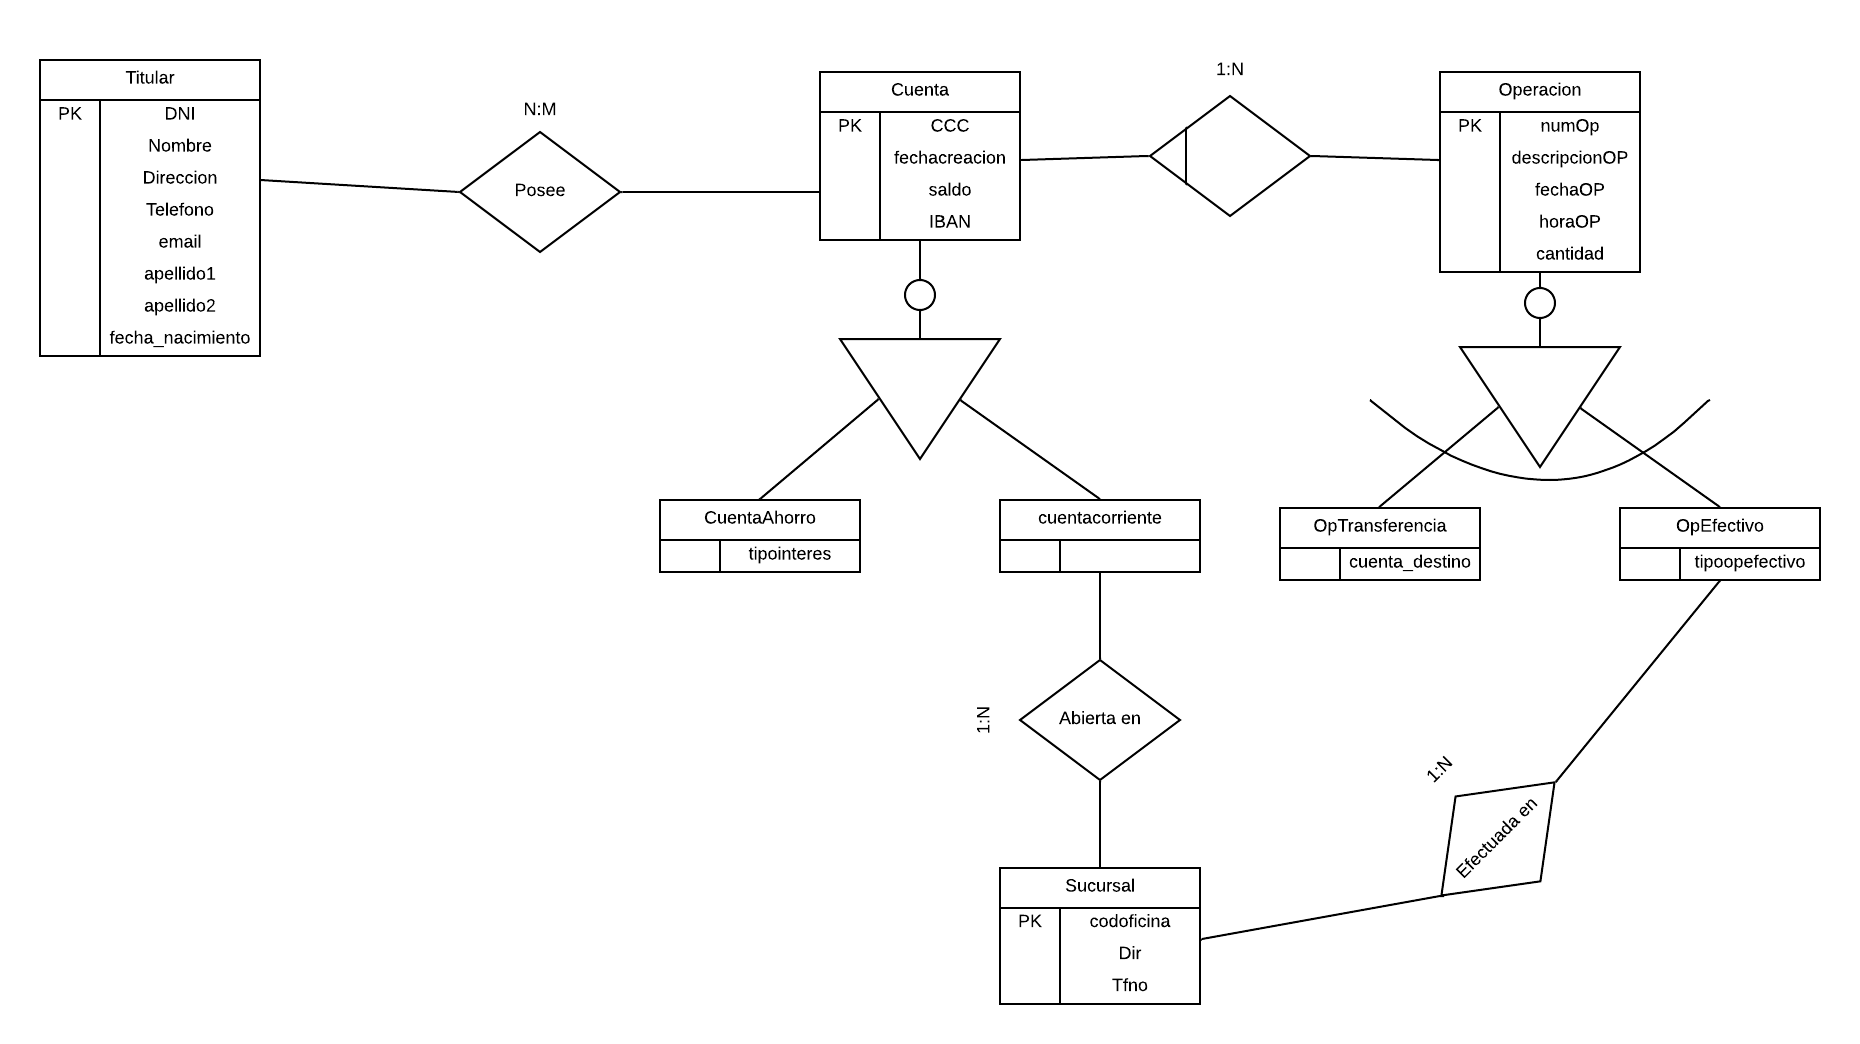
\includegraphics[scale=0.55]{images/DiagramaGLOBAL.png}
\label{fig:er_banquete}
\caption{Diagrama E/R de la base de datos de Banquete}
\end{figure}\\

La entidad \emph{Titular} es la que recogerá a todos los clientes de ambas bases, y contendrá toda su información, incluyendo la \textit{direccion}. Se ha optado por introducir este dato como un atributuo más de la tabla en lugar de crear una entidad con las direcciones. La dirección contendrá la calle, el piso, número y código postal. En el caso de \emph{Banquito} venía en un atributo, pero en el caso de \emph{Banquete}, se disponía en dos entidades, \textit{Dirección} y \textit{CodPostal}, esto se ha unificado en un atributo a través de la consulta ralizada a la hora de crear la vista con la siguientes sentencias:

\begin{lstlisting}
CREATE OR REPLACE VIEW titular_view AS
(
	-- BANQUITO
	-- Seleccionamos los atributos que queremos mostrar con sus respectivos
	-- nombres
	SELECT c.DNI as DNI, 
		c.nombre as NOMBRE,
		regexp_substr(c.apellido, '^[a-zA-Z]+\w|^[a-zA-Z]+$') APELLIDO1,
		regexp_substr(c.apellido, ' .*$') APELLIDO2,
		c.direccion as DIRECCION,
		TO_CHAR(c.telefono) as TELEFONO,
		c.email as EMAIL, 
		-- calculamos la edad ya que no disponemos de la fecha de 
		-- nacimiento, sino la edad en el momento de registro
		TO_DATE(sysdate-c.edad*365) as FECHA_NACIMIENTO
	FROM Cliente c
)
UNION
(
	-- BANQUETE
	-- Seleccionamos los atributos que queremos mostrar con sus respectivos
	-- nombres
	SELECT	t.DNI as DNI,
	t.nombre as NOMBRE, 
		t.apellido1 as APELLIDO1,
		t.apellido2 as APELLIDO2,
		d.calle || ', numero ' || d.numero || ', piso ' || d.piso 
			|| ', ' || d.ciudad || ', '
			|| (
				-- buscamos en codpostal el código correspondiente
				-- a la calle y ciudad que estamos mostrando
				SELECT distinct cp.codpostal 
				FROM codpostal@schema2bd2 cp 
				WHERE cp.calle = d.calle AND
					cp.ciudad = d.ciudad
			) 
			as DIRECCION,
		t.telefono as TELEFONO,
		-- no disponen de atributo email en banquete
		null as EMAIL,
		t.fecha_nacimiento as FECHA_NACIMIENTO
	FROM titular@schema2bd2 t 
		JOIN direccion@schema2bd2 d ON
			t.direccion = d.id_direccion
);
\end{lstlisting}
Para \emph{Banquito }simplemente se cogen los datos de la tabla \textit{Cliente} y se nombra las columnas siguiendo el esquema de \emph{Banquete}, de esta manera sus usuarios se sentirán mas cómdos. En cambio en la consulta a \emph{Banquete}, debemos realizar un \textit{join} con la tabla \textit{dirección} y  \textit{titular}, ya que el último contiene una clave ajena de dirección. Para obtener la dirección completa se concatenan los atributos de la tabla y para obtener el código posta, se hace a través de una consulta con la ciudad y la calle deseada.\\

La entidad \emph{Cuenta} contendrá tanto las cuenta corrientes como las cuentas de ahorro. Esta dispone de una relación \textit{posee} con titular con cardinalidad N:M, con esta relación vinculamos las cuenta con sus titulares. Para ello se realiza la siguiente vista:\\
\begin{lstlisting}
CREATE OR REPLACE VIEW Posee_view AS
    (
        SELECT p.DNI as TITULAR, to_char(p.Num_cuenta) AS CCC
        FROM Poseer p
    )
    UNION
    (
        select c1.titular, c1.CCC
        from cuenta@schema2bd2 c1
    );
\end{lstlisting}
Se realiza una unón con la tabla \textit{cuenta} de \emph{Banquete} y \textit{posee} de \textbf{Banquito}. \emph{Banquete} en su tabla \textit{cuenta } dispone de un atirbuto \textit{titular} que es el DNI del cliente al que pertenece esa cuenta (debido a la realación 1:N entre titular y cuenta). Para \emph{Banquito}  se ha tenido que obtener de la realación N:M posee que contine los DNIs asociados a sus cuentas.
 
\section{Parte 2 - Enunciado de un problema de diseño de bases de datos}

Se desea diseñar una base de datos para gestionar la información inherente a un hospital. En el hospital trabajan médicos y enfermeros. Los médicos tienen asignados una serie de pacientes. Los enfermeros tienen asignada una planta.\\
%Los pacientes ingresan en el hospital a partir del servicio de urgencias, y tras examinarles se les asigna a una planta.\\
La información sobre los trabajadores del hospital deberá contener información sobre su DNI, nombre, apellidos, fecha de nacimiento, dirección, teléfono de contacto. Los médicos deberán almacenar su especialidad y su número de colegiado. Los enfermeros almacenarán el servicio al que están asignados (planta, hematología, diálisis...).\\
Nuestro hospital está dividido en plantas, cada planta alberga pacientes ingresados y almacena la información relativa al uso destinado para esa planta.\\
Los pacientes almacenan su DNI, nombre, apellidos, fecha de nacimiento, dirección y teléfono. Disponemos de un historial clínico que almacena la información sobre los diagnósticos realizados a los pacientes.

\textbf{Poner aqui ese enunciado que hemos redactado}

\section{Parte 2- Esquema conceptual para el problema enunciado}

Para la realización del esquema conceptual de este problema, y pensando en su futura tarea de integración, se han realizado dos esquemas conceptuales con una semántica similar para el problema descrito anteriormente. Se ha tomado esta decisión para dificultar la tarea de integración entre las dos bases de datos.\\
El primer diagrama \textbf{{\LARGE Lo hacen Chus y Tambo asi que les toca a ellos}}.\\

El segundo diagrama (Figura \ref{fig:er_parte2_2}) refleja el problema enunciado anteriormente. En el mismo podemos observar que debido a que los médicos y enfermeros comparten ciertos atributos (\emph{DNI}, Nombre, apellidos, dirección, teléfono...) se ha llegado a la conclusión de que debía existir una entidad común, \emph{Personal}.\\
Por otra parte, los diagnósticos realizados por los pacientes forman su historia clínica. La entidad \emph{Diagnóstico} es una entidad débil ya que depende en identificación y en existencia de \emph{Paciente}.\\
Los pacientes ingresan en plantas, por lo tanto, se ha diseñado una entidad \emph{Ingreso} que refleja el ingreso de un paciente determinado en una planta determinada. Esta entidad es débil ya que un paciente puede encontrarse con varios ingresos a lo largo de su vida. Por lo tanto, un ingreso depende de la planta, el paciente y, las fechas de ingreso y de alta.\\
Dado que los médicos tienen varios pacientes, y un paciente puede tener varios médicos, se ha diseñado una relación \emph{M:N} entre \emph{Médicos} y \emph{Pacientes}.

\textbf{Poner aquí los dos esquemas ER y explicar que se ha tomado esta decisión para dificultar la integración.}

\section{Parte 2 - Esquema lógico 1 para el problema enunciado}

\textbf{Pues explicar las decisiones de diseño de este (CHUS Y RATAMBO).}

\section{Parte 2 - Esquema lógico 2 para el problema enunciado}

\textbf{Pues explicar las decisiones de diseño de este (PEDRO Y HAYK).}

\section{Parte 2 - Esquema global y su implementación en PostgreSQL}

\textbf{Puse aquí tenemos la incertidumbre de si querrán que sean vistas o una base de datos completa, pero de todas formas habrá que explicar las decisiones de diseño.}

\section{Actualizaciones de datos sobre el esquema global}

\textbf{Viabilidad? Pues depende de dónde quieras guardarlo. Pero esto habrá que hablar.}

\newpage
\section{Apéndice 1: Figuras}

\begin{landscape}
\begin{figure}
\centering
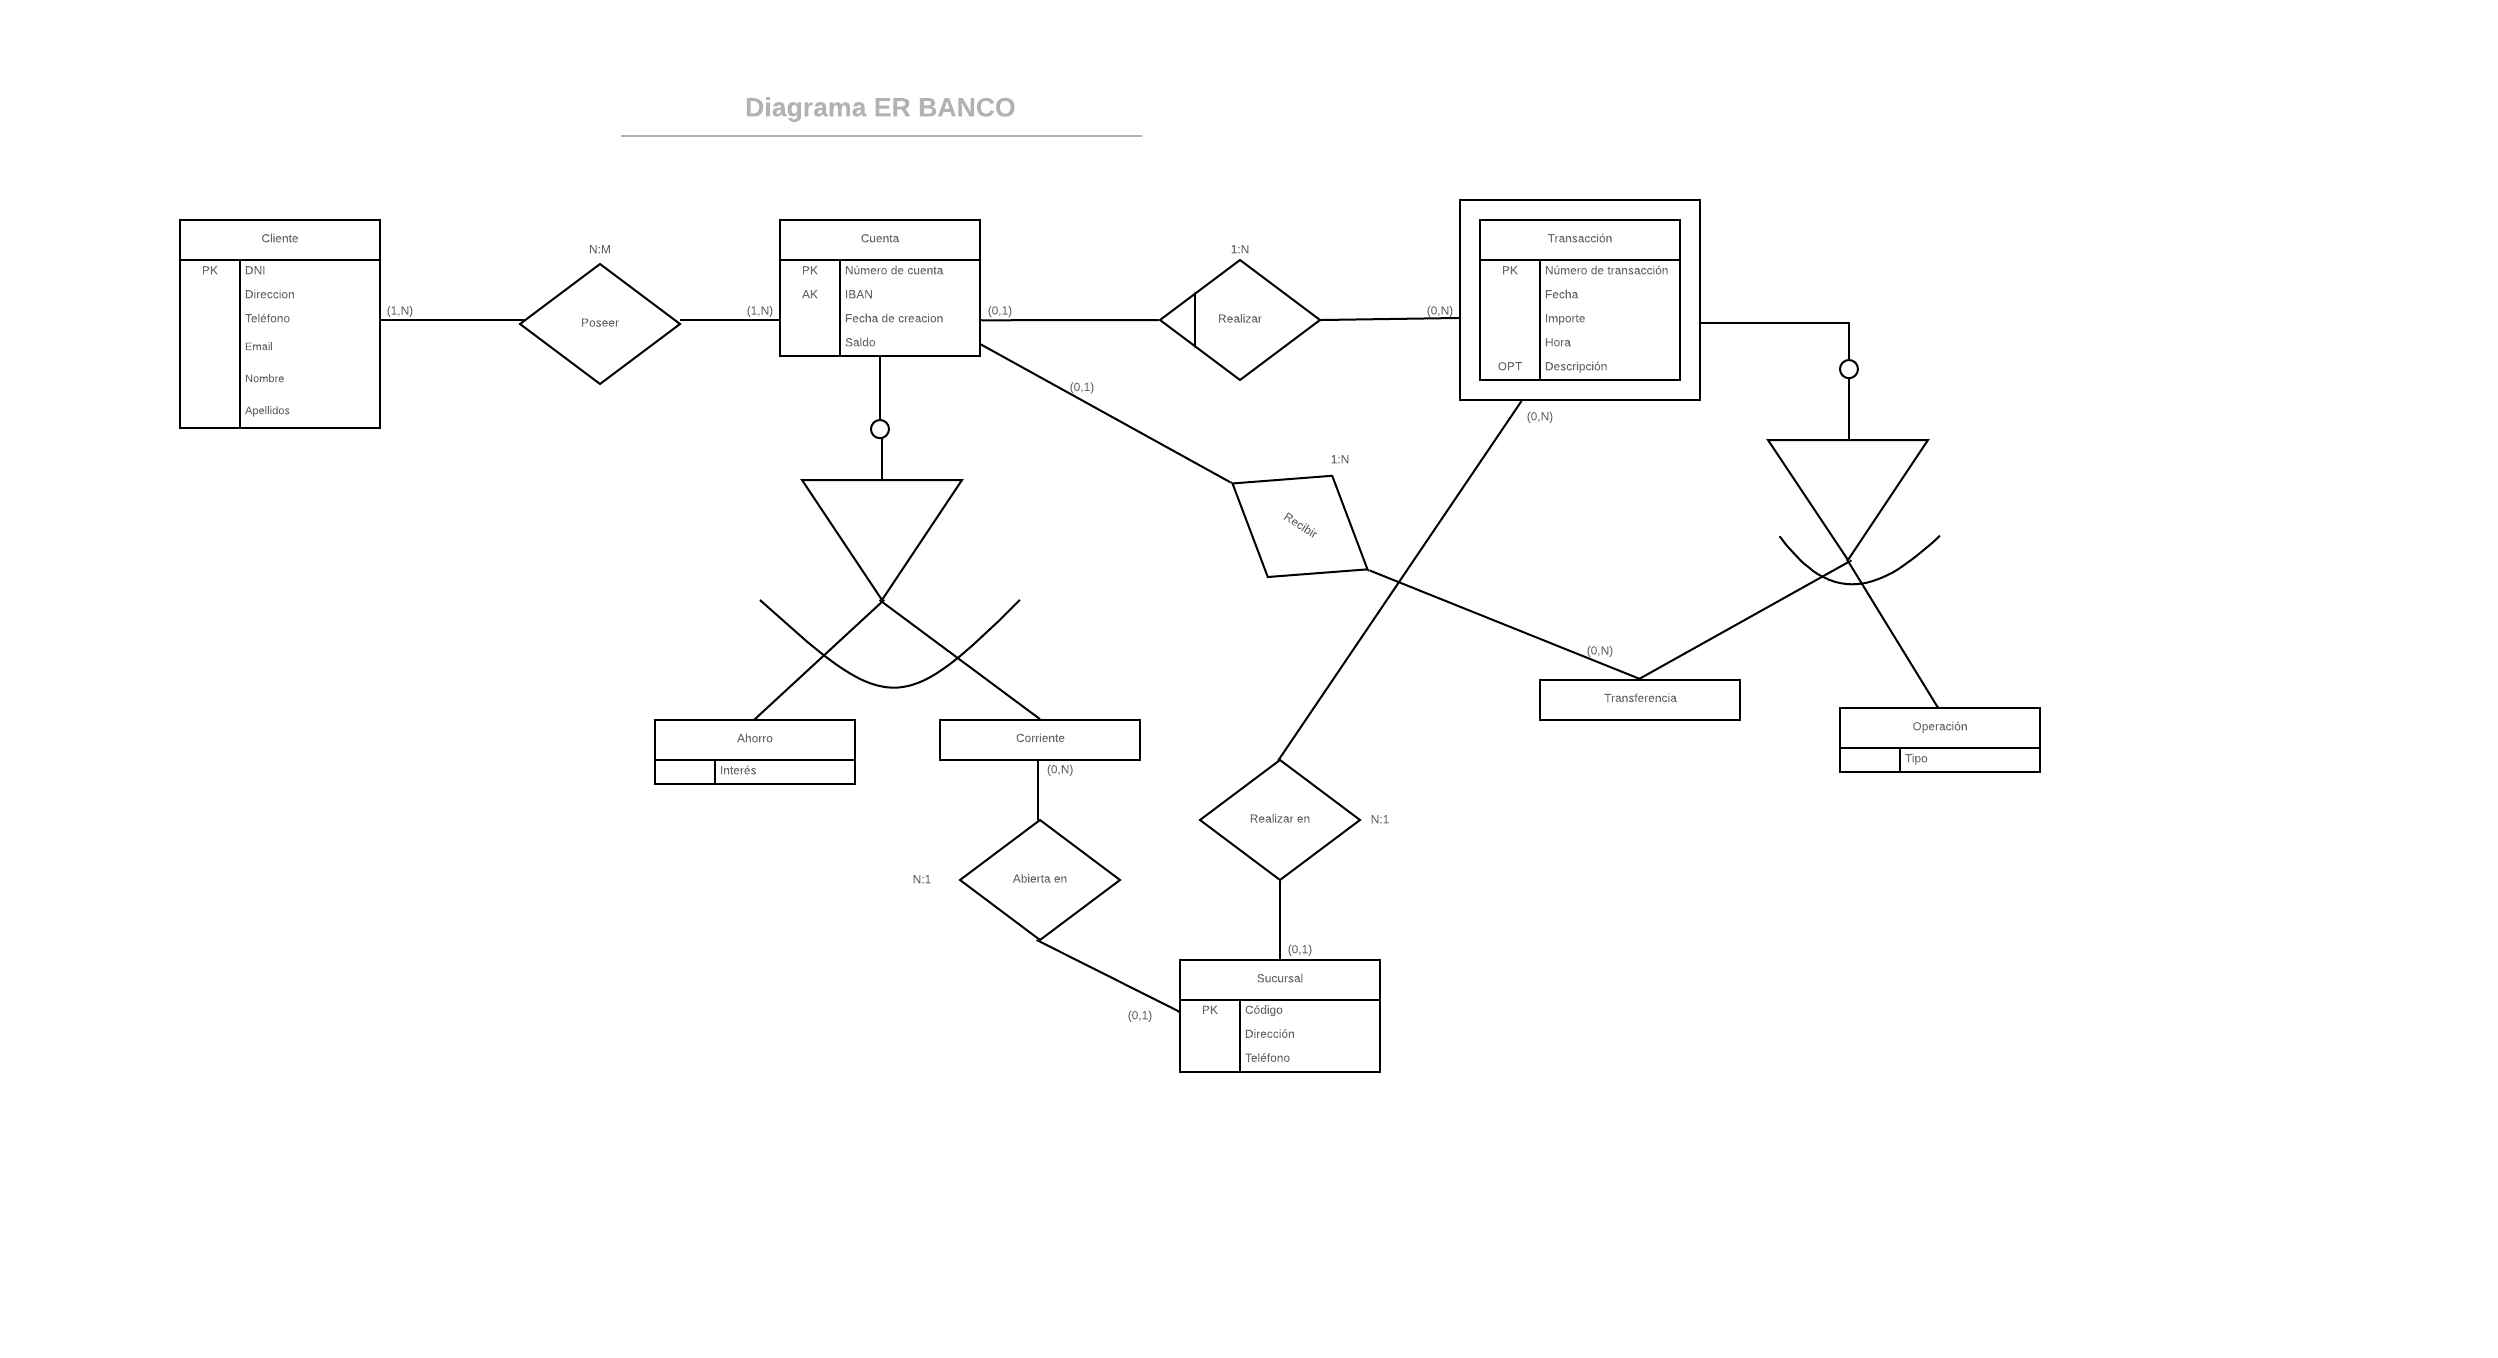
\includegraphics[scale=0.75]{images/er_practica1.png}
\caption{Esquema ER de la base de datos diseñada en la práctica 1}
\label{fig:er1}
\end{figure}
\end{landscape}


\begin{landscape}
\begin{figure}
\centering
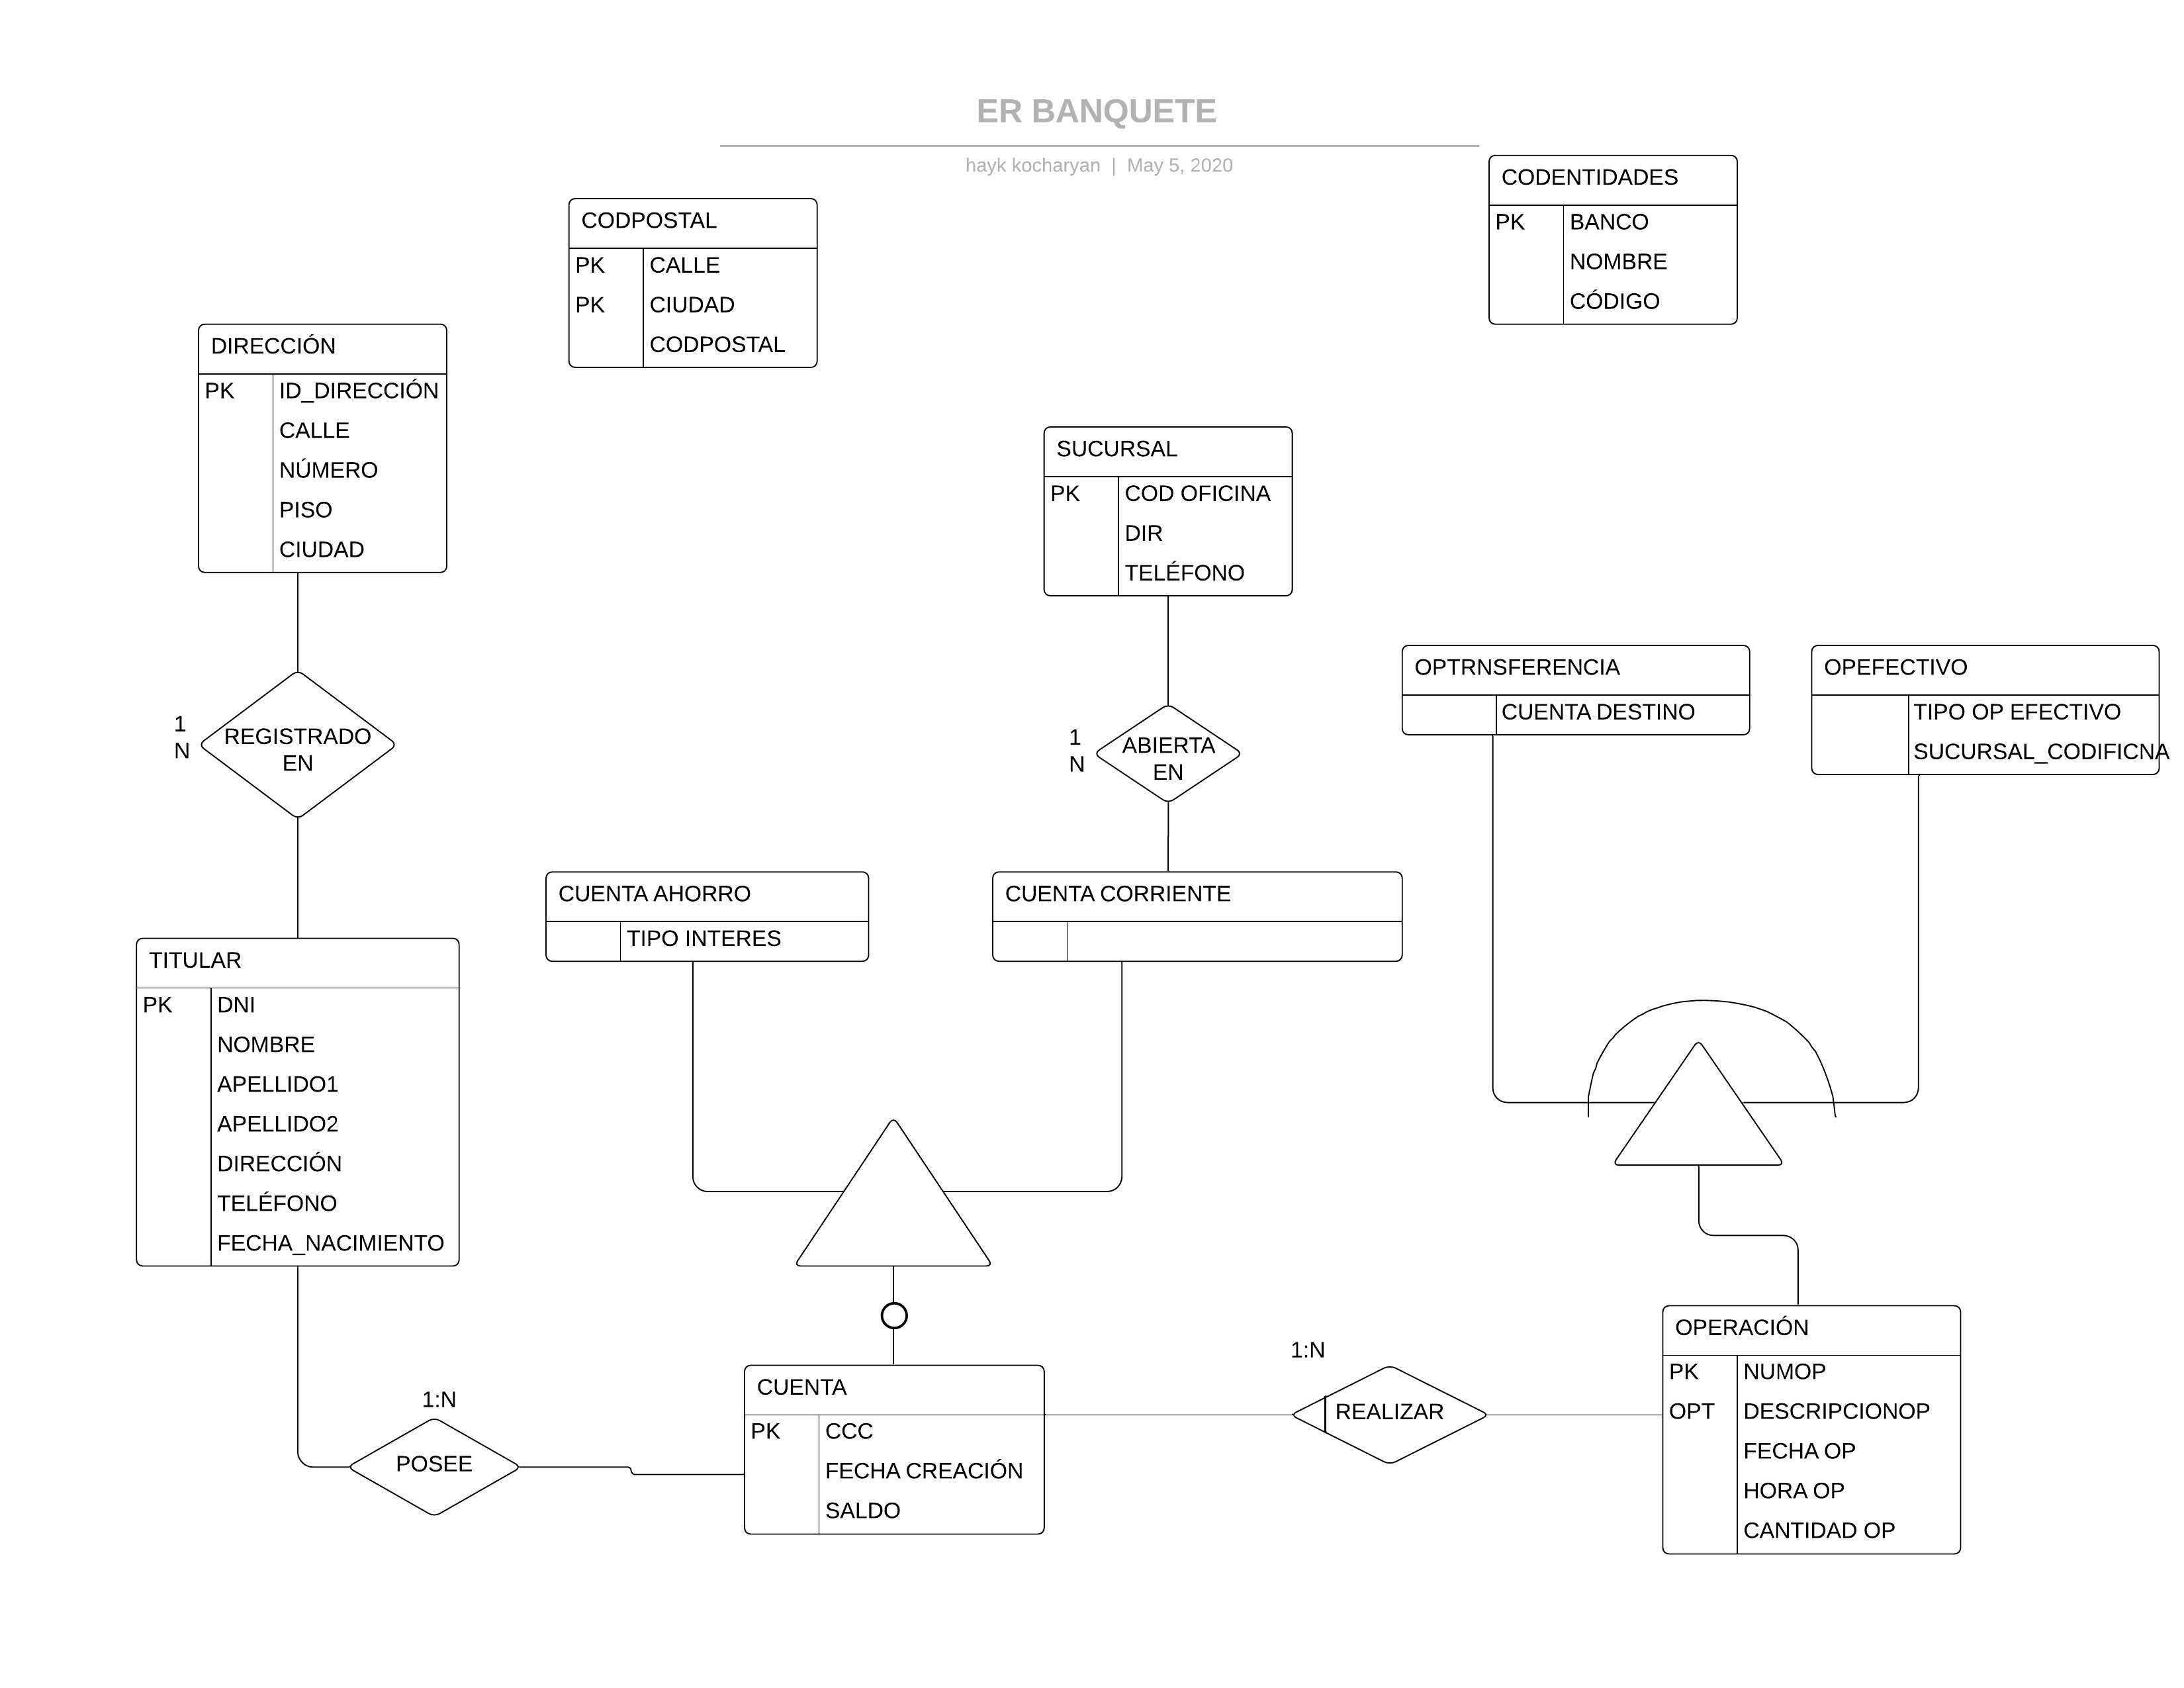
\includegraphics[scale=0.75]{images/ER_BANQUETE.jpeg}
\label{fig:er_banquete}
\caption{Diagrama E/R de la base de datos de Banquete}
\end{figure}
\end{landscape}


%% DIAGRAMAS PARTE 2

\begin{figure}
\centering
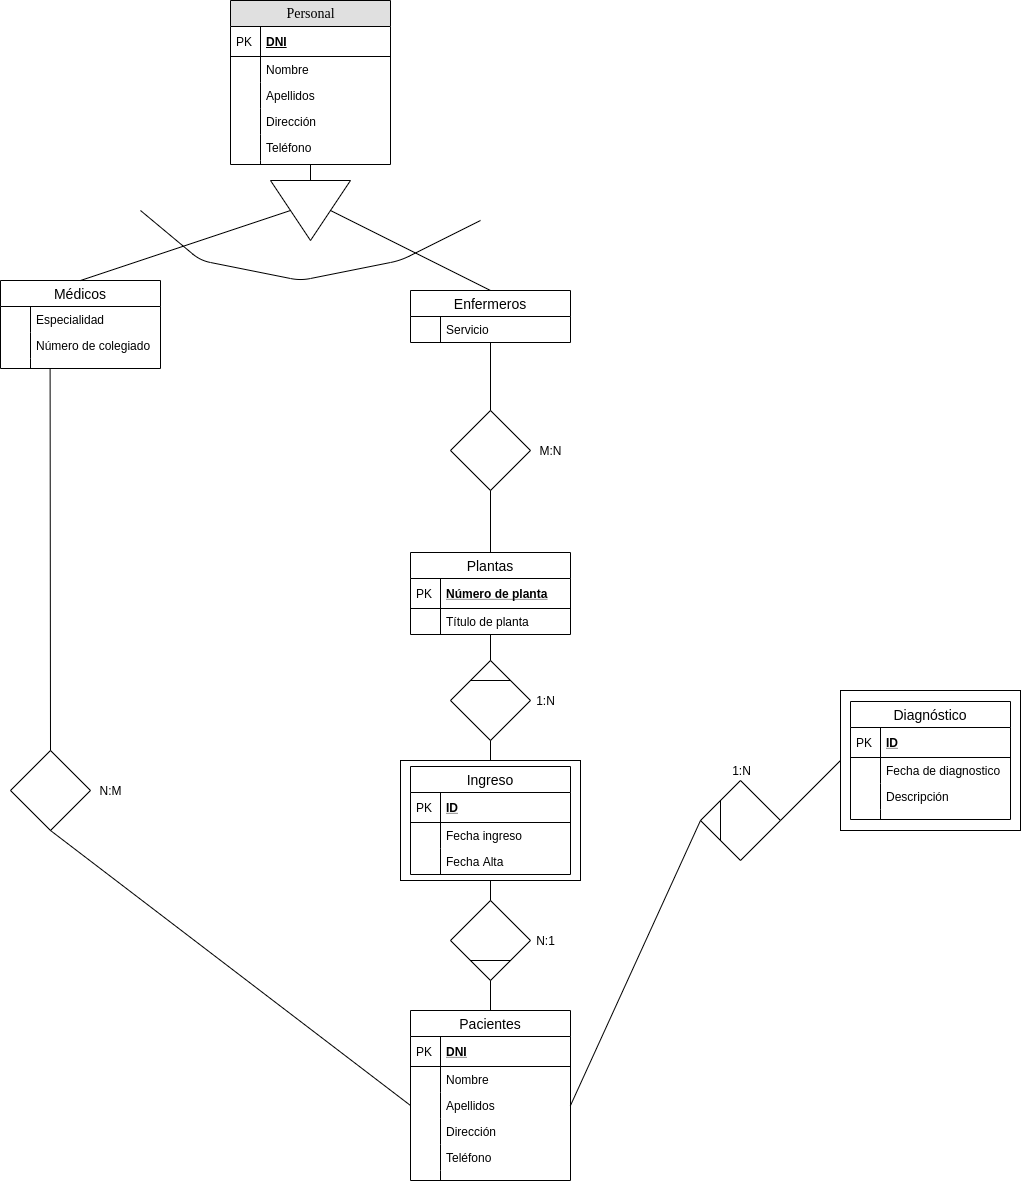
\includegraphics[scale=0.5]{images/er_parte2_2.png}
\label{fig:er_parte2_2}
\caption{Diagrama ER sobre el problema descrito en la parte 2}
\end{figure}



\end{document}
